% Figure 2: a chatbot (large language model) versus a tabular foundation model.
% Build: xelatex fig2_chatbot_vs_tfm.tex
\documentclass[border=2pt]{standalone}
\usepackage{fontspec}
\setmainfont{Times New Roman}
\usepackage{tikz}
\usetikzlibrary{positioning,arrows.meta,shapes.callouts,calc}
\definecolor{ink}{HTML}{222222}
\definecolor{llm}{HTML}{6E6E6E}
\definecolor{tfm}{HTML}{E69F00}
\definecolor{soft}{HTML}{F4F4F4}

\tikzset{
  head/.style={font=\small\bfseries, anchor=south},
  engine/.style={draw=#1, line width=0.9pt, rounded corners=3pt, fill=#1!12, minimum width=4.4cm,
                 minimum height=1.25cm, align=center, font=\footnotesize, text width=4.2cm},
  flow/.style={-{Stealth[length=2.2mm]}, line width=0.8pt, draw=ink!70},
  lab/.style={font=\scriptsize, text=ink!70, align=center},
}

\begin{document}
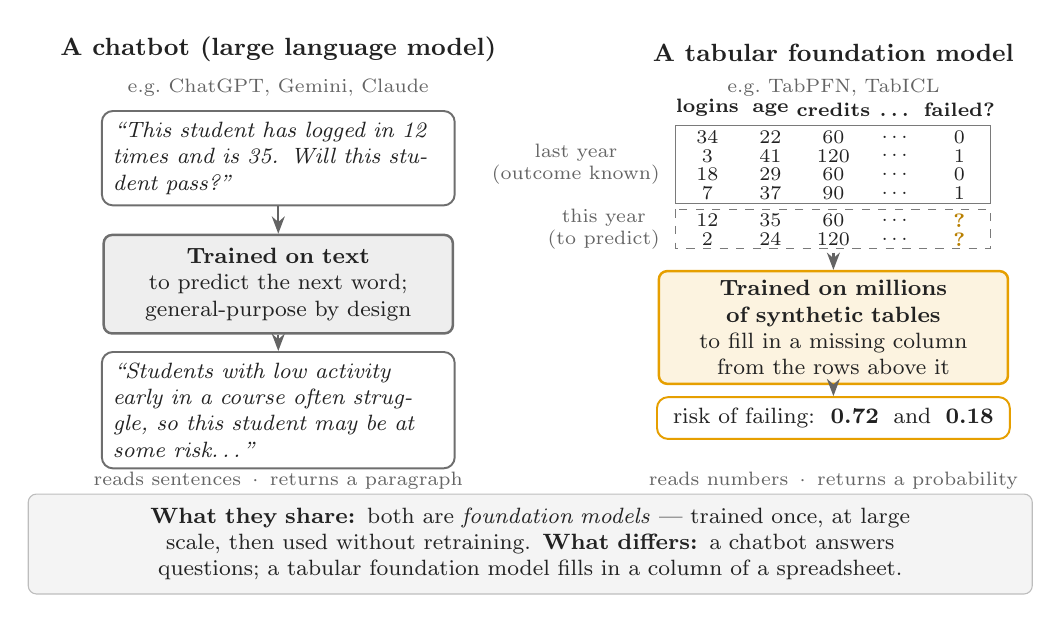
\begin{tikzpicture}[text=ink]

% =============================================================== chatbot
\begin{scope}[shift={(0,0)}]
\node[head] at (2.2,4.25) {A chatbot (large language model)};
\node[lab] at (2.2,4.05) {e.g.\ ChatGPT, Gemini, Claude};
% the question, as a speech bubble
\node[draw=llm, line width=0.7pt, rounded corners=4pt, fill=white, text width=4.2cm, align=left,
      font=\footnotesize\itshape, inner sep=4pt] (q) at (2.2,3.15)
  {``This student has logged in 12 times and is 35. Will this student pass?''};
\node[engine=llm] (e1) at (2.2,1.55) {\textbf{Trained on text}\\ to predict the next word;\\ general-purpose by design};
\node[draw=llm, line width=0.7pt, rounded corners=4pt, fill=white, text width=4.2cm, align=left,
      font=\footnotesize\itshape, inner sep=4pt] (a) at (2.2,-0.05)
  {``Students with low activity early in a course often struggle, so this student may be at some risk\ldots''};
\draw[flow] (q) -- (e1);
\draw[flow] (e1) -- (a);
\node[lab] at (2.2,-0.95) {reads sentences \,$\cdot$\, returns a paragraph};
\end{scope}

% =============================================================== tabular foundation model
\begin{scope}[shift={(6.3,0)}]
\node[head] at (2.95,4.25) {A tabular foundation model};
\node[lab] at (2.95,4.05) {e.g.\ TabPFN, TabICL};
% the input: last year's table plus this year's rows with the outcome missing
\def\cw{0.8}\def\rh{0.24}\def\xo{0.95}
\foreach \c/\t in {0/logins,1/age,2/credits,3/\ldots,4/failed?} {
  \node[font=\scriptsize\bfseries, anchor=south] at (\xo+\c*\cw+\cw/2,3.56) {\t};
}
\foreach \r/\v in {0/{34,22,60,\ldots,0},1/{3,41,120,\ldots,1},2/{18,29,60,\ldots,0},3/{7,37,90,\ldots,1}} {
  \foreach \x [count=\c from 0] in \v {
    \node[font=\scriptsize] at (\xo+\c*\cw+\cw/2,3.42-\r*\rh) {\x};
  }
}
\draw[ink!60, line width=0.4pt] (\xo,3.56) rectangle (\xo+5*\cw,2.58);
\node[lab, anchor=east] at (\xo-0.08,3.07) {last year\\(outcome known)};
\foreach \r/\v in {0/{12,35,60,\ldots},1/{2,24,120,\ldots}} {
  \foreach \x [count=\c from 0] in \v {
    \node[font=\scriptsize] at (\xo+\c*\cw+\cw/2,2.36-\r*\rh) {\x};
  }
  \node[font=\scriptsize\bfseries, text=tfm!80!black] at (\xo+4*\cw+\cw/2,2.36-\r*\rh) {?};
}
\draw[ink!60, line width=0.4pt, dashed] (\xo,2.5) rectangle (\xo+5*\cw,2.0);
\node[lab, anchor=east] at (\xo-0.08,2.25) {this year\\(to predict)};
\node[engine=tfm] (e2) at (2.95,1.0) {\textbf{Trained on millions of synthetic tables}\\ to fill in a missing column from the rows above it};
\draw[flow] (2.95,1.95) -- (e2);
% the output: one probability per new student
\node[draw=tfm, line width=0.7pt, rounded corners=4pt, fill=white, align=center, font=\footnotesize,
      text width=4.2cm, inner sep=4pt] (o) at (2.95,-0.15)
  {risk of failing:\, \textbf{0.72} \;and\; \textbf{0.18}};
\draw[flow] (e2) -- (o);
\node[lab] at (2.95,-0.95) {reads numbers \,$\cdot$\, returns a probability};
\end{scope}

% =============================================================== what they share
\node[draw=ink!30, fill=soft, rounded corners=3pt, text width=12.4cm, align=center, font=\footnotesize,
      inner sep=5pt] at (5.4,-1.75)
  {\textbf{What they share:} both are \emph{foundation models} --- trained once, at large scale, then used
   without retraining. \textbf{What differs:} a chatbot answers questions; a tabular foundation model fills
   in a column of a spreadsheet.};
\end{tikzpicture}
\end{document}
